% Chapter 4

\chapter{Experimental Results and Discussion} % Main chapter title

\label{Chapter4} % For referencing the chapter elsewhere, use \ref{Chapter3} 

\lhead{Chapter 4. \emph{Results}} % This is for the header on each page - perhaps a shortened title

%----------------------------------------------------------------------------------------
Malicious nodes detected properly by this simulation. When a blackhole node drops a packet the IDS detects the blackhole and gives output in the terminal.[\ref{fig:terminal}] And send the malicious node to the blacklist.

\section{Introduction}

In this simulation, blackhole node is detected in ns2. AODV is a reactive routing protocol. When the source node searches the route for communication. It sends RREQ to the neighbor nodes and sends the RREP to the route 1st hop. If 1st node drops the packet the message is sent to the admin that which node drop whose packet. A comparison between with and without blackhole is given in the table. \ref{tab:compare}

\begin{table}[]
	\centering
	\begin{tabular}{|l|l|l|}
		\hline
		\textbf{Parameter}          & \textbf{With Blackhole} & \textbf{Without Blackhole} \\ \hline
		Simulation  time in seconds & 7.969744514             & 7.996721981                \\ \hline
		Number of nodes             & 50                      & 50                         \\ \hline
		Number of sent packets      & 679                     & 1148                       \\ \hline
		Number of dropped packets   & 693                     & 616                        \\ \hline
		Average packet size         & 63.6649                 & 83.0259                    \\ \hline
		Number of dropped bytes     & 82048                   &           66566              \\ \hline
	\end{tabular}
	\caption{Simulation Comparison Of Blackhole Attack}
	\label{tab:compare}
\end{table}

%Figure   
\begin{figure}[htbp]
	\centering
	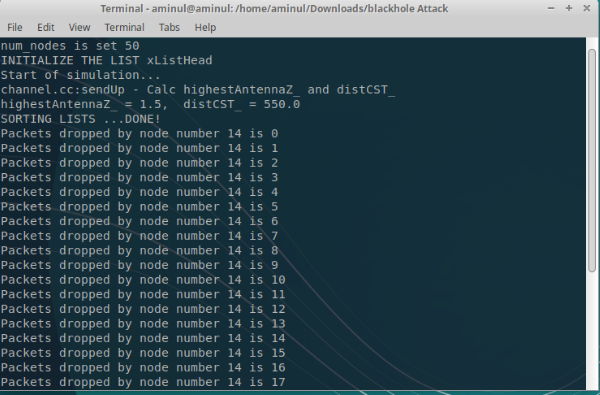
\includegraphics[scale=0.5]{out}
	\rule{35em}{0.5pt}
	\caption[Output in terminal]{Output in terminal}
	\label{fig:terminal}
\end{figure}
\pagebreak
\section{Experimental Results}
In this simulation 50 nodes is used and this simulation took place for around 8 min.
Both with and without blackhole nodes the simulation performed and observed the output.
It is observed that when the blackhole nodes are presented packet was sent in huge in number and drop rate is also higher. Throughput of generated packets are decreases almost 50\% less with 3 blackhole nodes among 50 nodes.\\

Three parameters are considered in this simulation.
They are:\\
1.Cumulative Sum\\
2.Throughput\\
3.Jitter
\subsection{Cumulative Sum}
It is a sequential analysis process. It is used to monitoring change detection. In a network, cumulative sum indicates the use of the network. when the malicious node is present the traffic of the network increases so the cumulative sum increased. \cite{gao2020cumulative}

% Please add the following required packages to your document preamble:
% \usepackage{multirow}
\begin{table}[]
	\begin{tabular}{|c|l|l|l|}
		\hline
		\textbf{Parameter}                 & \textbf{Nature} & \textbf{With Blackhole} & \textbf{Without Blackhole} \\ \hline
		\multirow{3}{*}{generated packets} & Minimum         & 1.00                    & 1.00                       \\ \cline{2-4}
		& Average         & 374.50                  & 583.50                     \\ \cline{2-4}
		& Maximum         & 748.00                  & 1166.00                    \\ \hline
		\multirow{3}{*}{sent packets}      & Minimum         & 1.00                    & 1.00                       \\ \cline{2-4}
		& Average         & 315.00                  & 560.50                     \\ \cline{2-4}
		& Maximum         & 629.00                  & 1120.00                    \\ \hline
		\multirow{3}{*}{forwarded packets} & Minimum         & 1.00                    & 1.00                       \\ \cline{2-4}
		& Average         & 19.50                   & 71.50                      \\ \cline{2-4}
		& Maximum         & 38.00                   & 142.00                     \\ \hline
		\multirow{3}{*}{received packets}  & Minimum         & 1.00                    & 1.00                       \\ \cline{2-4}
		& Average         & 630.00                  & 522.50                     \\ \cline{2-4}
		& Maximum         & 1259.00                 & 1044.00                    \\ \hline
		\multirow{3}{*}{dropped packets}   & Minimum         & 1.00                    & 1.00                       \\ \cline{2-4}
		& Average         & 347.00                  & 308.50                     \\ \cline{2-4}
		& Maximum         & 693.00                  & 616.00                     \\ \hline
	\end{tabular}
	\caption{Cumulative Sum Of Dropped Packets Simulation}
	\label{tab:sum}
\end{table}

%Figure   
\begin{figure}[htbp]
	\centering
	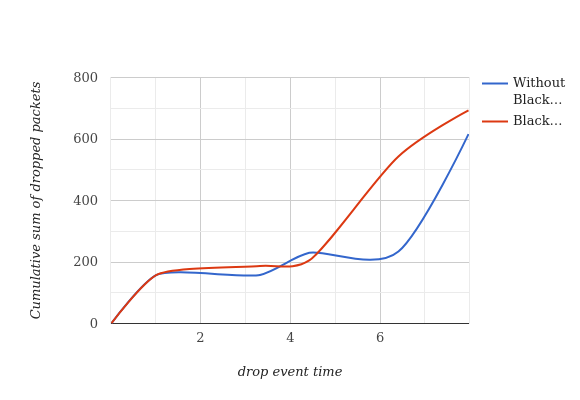
\includegraphics[scale=0.5]{sum}
	\rule{35em}{0.5pt}
	\caption[Cumulative sum of dropped packets]{Cumulative sum of dropped packets}
	\label{fig:sum}
\end{figure}


\subsection{Throughput}
It is a transmission measurement parameter. It is a ratio of transmitted traffic and unit of time. It is the best way of measuring a network. If the throughput is higher the traffic of the network is more. We should avoid a system with high traffic.

% Please add the following required packages to your document preamble:
% \usepackage{multirow}
\begin{table}[]
	\begin{tabular}{|c|l|l|l|}
		\hline
		\textbf{Parameter}                 & \textbf{Nature} & \textbf{With Blackhole} & \textbf{Without Blackhole} \\ \hline
		\multirow{3}{*}{generated packets} & Minimum         & 1.00                    & 1.00                       \\ \cline{2-4}
		& Average         & 83.11                   & 129.55                     \\ \cline{2-4}
		& Maximum         & 220.00                  & 220.00                     \\ \hline
		\multirow{3}{*}{sent packets}      & Minimum         & 1.00                    & 1.00                       \\ \cline{2-4}
		& Average         & 69.89                   & 124.44                     \\ \cline{2-4}
		& Maximum         & 165.00                  & 198.00                     \\ \hline
		\multirow{3}{*}{forwarded packets} & Minimum         & 0.00                    & 1.00                       \\ \cline{2-4}
		& Average         & 4.22                    & 15.78                      \\ \cline{2-4}
		& Maximum         & 17.00                   & 20.00                      \\ \hline
		\multirow{3}{*}{received packets}  & Minimum         & 1.00                    & 1.00                       \\ \cline{2-4}
		& Average         & 139.89                  & 116.00                     \\ \cline{2-4}
		& Maximum         & 256.00                  & 231.00                     \\ \hline
		\multirow{3}{*}{dropped packets}   & Minimum         & 1.00                    & 0.00                       \\ \cline{2-4}
		& Average         & 77.00                   & 68.44                      \\ \cline{2-4}
		& Maximum         & 204.00                  & 213.00                     \\ \hline
	\end{tabular}
	\caption{Throughput Of Dropping Packets Simulation}
	\label{tab:through}
\end{table}

%Figure   
\begin{figure}[htbp]
	\centering
	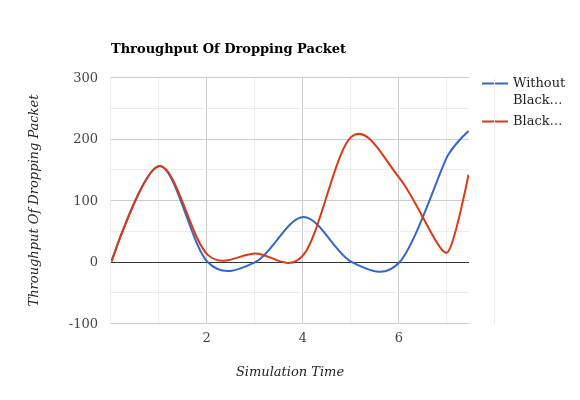
\includegraphics[scale=0.5]{through}
	\rule{35em}{0.5pt}
	\caption[Throughput Of Dropping Packet]{Throughput Of Dropping Packet}
	\label{Throughput Of Dropping Packet}
\end{figure}


\subsection{Jitter}
It is the variance in the time delay between a data packet over a network. It is defined as to disturb in normal packet sending sequence. Jitter helps in decision making about a network.


% Please add the following required packages to your document preamble:
% \usepackage{multirow}
\begin{table}[]
	\begin{tabular}{|c|l|l|l|}
		\hline
		\textbf{Parameter}                 & \textbf{Nature} & \textbf{With Blackhole} & \textbf{Without Blackhole} \\ \hline
		\multirow{3}{*}{generated packets} & Minimum         & -0.01                   & -0.01                      \\ \cline{2-4}
		& Average         & 0.11                    & 0.045                      \\ \cline{2-4}
		& Maximum         & 0.29                    & 0.28                       \\ \hline
		\multirow{3}{*}{sent packets}      & Minimum         & -0.01                   & -0.01                      \\ \cline{2-4}
		& Average         & 0.11                    & 0.04                       \\ \cline{2-4}
		& Maximum         & 0.29                    & 0.28                       \\ \hline
		\multirow{3}{*}{forwarded packets} & Minimum         & -0.01                   & -0.01                      \\ \cline{2-4}
		& Average         & 0.11                    & 0.05                       \\ \cline{2-4}
		& Maximum         & 0.28                    & 0.28                       \\ \hline
		\multirow{3}{*}{received packets}  & Minimum         & 0.01                    & 0.01                       \\ \cline{2-4}
		& Average         & 0.15                    & 0.20                       \\ \cline{2-4}
		& Maximum         & 0.37                    & 0.37                       \\ \hline
		\multirow{3}{*}{dropped packets}   & Minimum         & 0.00                    & 0.00                       \\ \cline{2-4}
		& Average         & 0.10                    & 0.14                       \\ \cline{2-4}
		& Maximum         & 0.40                    & 0.38                       \\ \hline
	\end{tabular}
	\caption{Jitter Of Dropped Packets Simulation}
	\label{tab:jitter}
\end{table}

%Figure   
\begin{figure}[htbp]
	\centering
	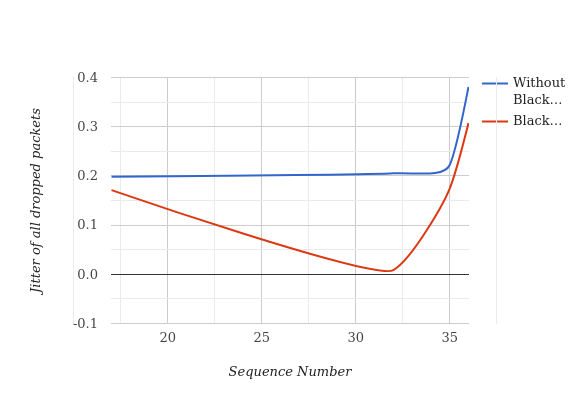
\includegraphics[scale=0.5]{jitter}
	\rule{35em}{0.5pt}
	\caption[Jitter Of Dropped Packets]{Jitter of dropped packets}
	\label{fig:jitter}
\end{figure}
\pagebreak\
\section{Descriptive Analysis}
50 nodes simulation when 3 of them are blackhole is observed. In this process of identification every node is observed. The network size doesn't matter in this case. Ad-hoc on demand routing is most used and efficient routing protocol. It is secured in nature. Result of this project is satisfectory.


\section{Summary}
It observed that the cumulative sum of packet dropping increases 12.66\% for 3 malicious nodes.\\At same way throughput of dropping packet increase by 12.51 \% \& average jitter of dropping a packet is increased by 40\%.